\documentclass[11pt]{article}

\usepackage[utf8]{inputenc}
\usepackage[T1]{fontenc}
\usepackage{lmodern}
\usepackage{amsmath,amsfonts}
\usepackage{subfigure}
\usepackage{bm}
\usepackage{listings}
\usepackage{pifont}%
\usepackage{hyperref}
\usepackage{enumitem}
\usepackage{amsmath,amsfonts,amssymb}

\usepackage{pgfplots,tikz}

\usepackage{fullpage}      % Margens
\usepackage{indentfirst}   % Autoidentar

\usepackage{graphicx}       % Pictures

\newlist{level}{itemize}{4}
\setlist[level]{label={},noitemsep,topsep=0pt}
\newcounter{algo}
\renewcommand{\thealgo}{\arabic{algo}.}
\newenvironment{algorithm}[1]{%
    \refstepcounter{algo}%
    \paragraph{Algorithm \thealgo}#1%
    \vspace{2pt}\hrule\vspace{5pt}%
    \begin{level}
}{%
    \end{level}%
    \vspace{5pt}\hrule\vspace{\baselineskip}%
}


\title{Bayesian Covariance Estimation for Kalman Filter based Digital Carrier Synchronization}

\author{Gerald LaMountain\\Department of Electrical and Computer Engineering\\Northeastern University\\Boston, Massachusetts}

\date{April 25, 2018}

\begin{document}

% \noindent Northeastern University
% \hfill March 29, 2018

% \noindent Department of Electrical and Computer Engineering
% \hfill EECE5698-ST (Spring 2018)

% \noindent {} \hfill \textbf{Final Project}

% \noindent \rule{\linewidth}{1.5pt}

% \vspace*{.5cm}

\maketitle

% \underline{Due date}: Wednesday 25, April 2018. No extension will be granted. Send your report to closas@northeastern.edu
% 
% To complete the project, feel free to consult other sources (i.e., books, internet, etc.) besides class notes or suggested references. Justify your answers!
% 
% \noindent \rule{\linewidth}{1pt}
% \vspace*{.15cm}
% 
% The objective of the EECE5698's Final Project is to learn more about certain aspects of the materials covered in class. Topics can be proposed by you, but a list of suggested topics is provided below for your reference and choice.  Some proposed topics contain a reference article, which is not the unique source of information, consider that as a starting point and dig deeper in the literature to have a broader understanding of the matter. 

\section{Overview}

One of the critical steps of the GNSS receiver is carrier synchronization, where after the acquisition stage of the receiver computes the cross ambiguity function and detects any usable satellites, the system must track the time-varying code delay, carrier phase and carrier Doppler frequency for the signals recieved from each detected satellite. These parameters are used to correctly demodulate the navigation message and obtain the pseudoranges to the different satellites in view. While standard receivers rely on code-based positioning, carrier phase is of particular interest in modern carrier phase-based positioning techniques such as real-time-kinematic (RTK) and precise-point-positioning (PPP), used in high-precision GNSS receivers. Synchronization is a challenging task under harsh propagation conditions such as multipath, non-line-of-sight (NLOS), high-dynamics, shadowing, strong fadings or ionospheric scintillation. These non-nominal propagation conditions affect differently the code and carrier synchronization stages. While multipath and NLOS clearly impair code tracking, high-dynamics and ionospheric scintillation mainly affect carrier tracking. %In general, carrier synchronization tends to be more sensitive than time-delay tracking.

Standard mass-market GNSS receivers' synchronization rely on well-known delay-locked loop (DLLs), phase-locked loop (PLL) and frequency-locked loop (FLL) architectures, inherited from the analog era. The performance obtained with such techniques is good enough in benign propagation scenarios, but typically deliver poor performances under harsh propagation conditions. Both code and carrier tracking, or the joint code/carrier synchronization, can be formulated as an estimation problem, which can be solved using Bayesian filtering methods. The Kalman filter (KF) is the optimal analytical solution for linear/Gaussian systems, but suboptimal algorithms must be considered in nonlinear and/or non-Gaussian scenarios. The most popular solution for nonlinear/Gaussian systems is the extended KF (EKF), which linearizes the possibly nonlinear process or measurement functions and applies the standard linear KF equations.
% To avoid such linearization, which can be challenging in highly nonlinear scenarios, we can consider sigma-point Gaussian filters (SPGFs), or even more advanced techniques such as sequential Monte Carlo methods (a.k.a Particle Filters) in non-Gaussian scenarios. 
In the GNSS literature, it has been shown that KF-based synchronization solutions \cite{Vila17c} may overcome the performance limitations of standard approaches. The main advantages of the KF over DLL/PLL/FLL architectures are: i) it is formulated from an optimal filtering standpoint, ii) it has an implicit adaptive filter bandwidth \cite{Vila-14a}, and iii) a nonlinear KF (i.e., EKF or SPGF) allows us to avoid the problems associated with the use of code, phase or frequency discriminators \cite{Vila-14b}. On the other hand, Kalman filters are not as easy to tune and require more parameters than standard closed-loop techniques. One of the main practical disadvantages of KF-based techniques in many practical contexts, including GNSS synchronization, is that the model noise statistics (i.e., process and measurement noise covariance matrices) may not be known a priori. Of particular interest in the GNSS synchronization context are the measurement noise statistics, which may vary with a number of different factors including time and location. Although it may be possible to achieve fairly strong filter performance using a suitable a priori estimate of the unknown statistical parameters, methods have been proposed for estimating these parameters from measured data within the Kalman filter framework \cite{Dunik17a}.

In this paper, we will discuss the implementation of a nonlinear state space model for the time evolution of carrier phase and doppler shift parameters within the GNSS reciever, as well as the implementation of an Extended Kalman Filter for tracking these parameters based on noisy measurements modeled after those which we would expect to receive from the acquisition step of the receiver. Using data simulated according to the nonlinear state space model, we will evaluate the performance of this filter using different estimates of the "unknown" measurement noise statistics. Finally, we will, propose, implement and finally test a method for online estimation of the measurement noise covariance based on Bayesian inference, which provides several possible advantages over those methods described in the literature.

% is that their performance is typically shown only in controlled simulated scenarios, because their implementation and testing is more complex than using standard techniques (i.e., to use a standard PLL we only need to specify a few well-understood parameters such as the loop bandwidth or the damping factor). This typically prevents potential users to consider these techniques for real-life scenarios, and then it is not easy to judge their potential benefit for new applications. To improve GNSS availability in challenging propagation scenarios or its use for new scientific applications, it is of capital importance to be able to test the performance of such Bayesian filtering techniques using accepted models of carrier phase time evolution. 

\section{Carrier Phase Tracking using Kalman methods}

\subsection{Introduction to Carrier Synchronization}

Carrier synchronization is a process which is not unique to GNSS applications, but rather a critical component of the receiver of any digital communication system which relies on coherent signal detection. Propagation of a transmitted signal through an imperfect or complex channel results in disturbances to the carrier phase, time-delay and amplitude of the signal, which must be known if the transmitted information is to be recovered at the receiver. Generally, parameters characterizing these disturbances are time-varying and unknown to the receiver, and must be estimated and tracked based only on the received signal. In the GNSS receiver, information about the time-varying code delay, carrier phase and carrier Doppler frequency are needed to correctly demodulate the navigation message and obtain the observables used to compute an estimate of the position of the receiver. The method of determining pseudoranges based on carrier phase measurement is known as carrier-phase tracking, and is used in high-end GNSS receivers to deliver subdecimetric level positioning accuracy.

\subsection{Traditional methods for Carrier Synchronization}

By far the most widely used technique used for phase tracking in both the analogue and digital domains is the phase-locked loop (PLL). The PLL is a traditionally analogue control system developed in the early 20th century for synchronizing the phase of the signal produced by a local oscillator with a signal received over an analogue wireless or cable transmission line. As technology has transitioned into the digital domain, applications for digital phase synchronization have become numerous, leading to the development of hardware and software based digital PLL systems. The principle operation of a phase locked loop is as follows \cite{Best-07}:

\begin{enumerate}
  \item The received signal is processed through a phase detector, or discriminator, which produces an output with amplitude proportional to the difference between the output and input phase of the system, called the error signal.
  \item The error signal is filtered through a low pass filter called a loop filter, which smooths the error signal to produce a suitable control signal for the oscillator.
  \item The smoothed error signal is added to the controlling input of the variable frequency oscillator to drive the phase of the oscillator output to match that of the received signal.
  \item Finally, the output of the oscillator is fed back to the second input phase detector and the process is repeated.
\end{enumerate}

In the context of GNSS synchronization, PLL architectures are suited for performing Doppler shift tracking, however a variation of the PLL known as the Delay-Locked Loop (DLL) is required for performing code error tracking. A DLL functions similarly to a PLL, with the exception that it uses a variable delay line in the place of a variable frequency oscillator, which produces a local code replicas which are properly time aligned with the incoming signal so as to maximize correlator accuracy.

PLLs and DLLs may be combined into more complicated synchronization architectures which improve stability and provide better performance and accuracy under low signal conditions, however these architectures are limited in their ability to track signal parameters under high dynamic conditions. Furthermore, these architectures are limited to a fixed bandwidth, which limits their adaptability to changing conditions. Although research has been done into adaptive PLL-based architectures which provide valuable features such as variable bandwidth and adaptations for high dynamic conditions \cite{Fant-12}\cite{Ward-98}\cite{Leg00}, modern signal processing techniques have been developed since the advent of the phase locked loop which have been shown to have significant advantages over these classical techniques.

\subsection{Kalman Filtering Methods for Carrier Synchronization}

The operation performed by a traditional PLL/DLL based carrier synchronization loop can be viewed as a parameter estimation and tracking operation: the time-varying parameters of the transmitted signal are estimated from the received signal, and those parameters are in turn used to synchronize the system to the transmitted signal. Real-time optimal estimation of time-varying parameters in this way is what's known as \textit{recursive optimal filtering}. Optimal filtering in general has been the subject of much study throughout the latter half of the 20th century which has given rise to a number of real-time and batch optimal filtering techniques. Although these techniques differ in principle and function, they all aim to accomplish the same goal: given an appropriate model of a system, typically characterized through a state space representation, find statistically optimal estimates of the (possibly time-varying) parameters which characterize the state of the system at a given time. More technically speaking,

% \vspace*{.5cm}
\noindent Given a state space model of the form \begin{align}
&\mathbf{x}_k = \mathbf{f}_{k-1}(\mathbf{x}_{k-1}) + \bm{\nu}_{k-1}~, & & \bm{\nu}_{k-1}\sim \mathcal{N}(\mathbf{0},\mathbf{Q}_{k-1}), \label{eq:system_state} \\
&\mathbf{y}_k = \mathbf{h}_{k}(\mathbf{x}_{k}) + \mathbf{n}_{k} ~, & & \mathbf{n}_{k}\sim \mathcal{N}(\mathbf{0},\mathbf{R}_{k}), 
\label{eq:system_meas}
\end{align}
\noindent and measurements \small$\mathbf{y}_k \in \mathbb{R}^{n_y}$ \normalsize for all discrete sample times $k \in (-\infty,t]$, estimate the value of \small$\mathbf{x}_k \in \mathbb{R}^{n_x}$ \normalsize.
% \vspace*{.5cm}

By characterizing the time evolution of the carrier phase and Doppler shift parameters through a state space model, it is possible to use optimal filtering to perform the same carrier synchronization task as a PLL/DLL architecture.

\subsubsection{Introduction to Kalman Filtering and the Extended Kalman Filter}

Although the theory behind optimal filtering is rich and gives rise to numerous signal processing techniques, by far the most commonly known and popular state estimation algorithm is the Kalman filter due to its simplicity and effectiveness in many applications. There are several ways to derive the Kalman from the principles of optimal filtering, and while some of them are rather complex, the filter algorithm itself is rather simple:

\begin{algorithm}{Extended Kalman Filter Algorithm}\label{algo:ekf}
    \item \textbf{Initialize:}
    \item Set $\mathbf{\hat{x}}_{0|0}$ and $\mathbf{P}_{0|0}$ to the initial state and state covariance respectively.
    \item \textbf{for} k=1 to N \textbf{do}
    \begin{level}
        \item \textbf{Prediction Step:}
        \item Estimate the predicted state: $\mathbf{\hat{x}}_{k|k-1} = \mathbf{f}_{k}(\mathbf{\hat{x}}_{k-1|k-1})$
        \item Compute the Jacobian $\mathbf{F}_{k}$ of $\mathbf{f}_{k}(\mathbf{\hat{x}}_{k-1|k-1})$
        \item Estimate the predicted state covariance: $\mathbf{P}_{k|k-1} = \mathbf{F}_{k}(\mathbf{P}_{k-1|k-1})\mathbf{F}_{k}^* + \mathbf{Q}_{k}$
        \item \textbf{Measurement Step:}
        \item Estimate the predicted measurement: $\mathbf{\hat{y}}_{k|k-1} = \mathbf{h}_{k}(\mathbf{\hat{x}}_{k|k-1})$
        \item Compute the Jacobian $\mathbf{H}_{k}$ of $\mathbf{h}_{k}(\mathbf{\hat{x}}_{k|k-1})$
        \item Estimate the innovation covariance: $\mathbf{S}_{k|k-1} = \mathbf{H}_{k}(\mathbf{P}_{k|k-1})\mathbf{H}_{k}^* + \mathbf{R}_{k}$
        \item Estimate the Kalman gain: $\mathbf{K}_{k} = \mathbf{P}_{k|k-1}(\mathbf{H}_{k})\mathbf{S}_{k|k-1}^{-1}$
        \item Estimate the updated state: $\mathbf{\hat{x}}_{k|k} = \mathbf{\hat{x}}_{k|k-1} + \mathbf{K}_{k}(\mathbf{y}_k - \mathbf{\hat{y}}_{k|k-1})$
        \item Estimate the error covariance: $\mathbf{P}_{k|k} = \mathbf{P}_{k|k-1} - \mathbf{K}_{k}(\mathbf{H}_{k})\mathbf{P}_{k|k-1}$
    \end{level}
    \item end for
\end{algorithm}

\noindent The EKF algorithm, shown as Algorithm \ref{algo:ekf} provides an iterative method by which we can estimate parameters given noisy measurements and a nonlinear state space. Numerous resources are available for a more comprehensive explanation of the operation of the extended Kalman filter, but for the purposes of this work, we will focus on its application to carrier phase estimation. If we define our state vector to be comprised of the carrier phase offset (rads), Doppler shift (Hz) and Doppler shift rate (Hz/s), as $[\theta_k,\mathit{f_{d,k}},\mathit{f_{r,k}}]^\intercal$ according to the literature \cite{vila18}, we can define a linear state transition model:

% \vspace*{.5cm}
\begin{align}
&\mathbf{x}_k = \begin{pmatrix}
  1 & 2 \pi T_{s} & \pi T_{s}^{2} \\
  0 & 1 & T_s \\
  0 & 0 & T_{s}^{2}/2 
 \end{pmatrix}\mathbf{x}_{k-1} + \bm{\nu}_{k}~, & & \bm{\nu}_{k}\sim \mathcal{N}(\mathbf{0},\mathbf{Q}_{k}), \label{eq:system_state} \\
\end{align}

\noindent where $T_s$ is the time period between subsequent measurements $k-1$ and $k$. With measurement vector $[y_{i,k},y_{q,k}]^\intercal$ corresponding to the in-phase and quadrature components of the carrier phase offset, we define the nonlinear measurement model:

\begin{align}
&\mathbf{y}_k = \alpha_k \begin{bmatrix}cos(\theta_k)\\sin(\theta_k)\end{bmatrix} + \mathbf{n}_{k} ~, & & \mathbf{n}_{k}\sim \mathcal{N}(\mathbf{0},\mathbf{R}_{k}), 
\label{eq:system_meas}
\end{align}
% \vspace*{.5cm}

\noindent then application of appropriate measurements to an extended Kalman filter built around this model will produce estimates of the carrier phase offset, Doppler shift and Doppler shift rate at each time instance for each signal being tracked, thus satisfying the requirements of the estimation portion of the carrier synchronization component of the receiver.

\subsection{Kalman Filtering vs PLL Methods}

The literature contains comprehensive comparisons of PLL/DLL and Kalman filter architectures \cite{vila2017plls}. The first interesting point to note is that under optimal, steady-state conditions, a second-order Kalman filter is equivalent to a second-order PLL \cite{Pata-99}, and in fact, it can be shown that the PLL is a particular case of the general Kalman filter. This sets an important threshold for performance: under optimal, stationary conditions, the two methods are equivalent. However, under real-world conditions, the system may not tend towards a steady state but rather vary over time. In this sense, the Kalman filter, which updates its gain in a principled way based on the uncertainty in the measurements provided to the system, has an advantage over the PLL design which updates its gain based on a heuristic. Another metric under which the two methodologies may be compared are bandwidth trade-offs and adaptability. As described previously, traditional PLL architectures have a fixed bandwidth, which are tuned as part of the design of the system. Adaptive PLL architectures can be developed by changing parameters within the in a suboptimal manner based on predefined thresholds. By contrast, the Kalman filter has inherently adaptive bandwidth which is computed optimally under well defined noise characteristics $\mathbf{Q}_{k-1}$ and $\mathbf{R}_k$.

\subsection{Challenges and Limitations}

An attentive reader may note that a few of the variables needed for the application of the Kalman filter are not explicitly defined. First, the initial state of the system, may be initialized to zero with covariances provided by the output of the acquisition component of the receiver. Second, the value of $\alpha_k$ is left undefined, and must be estimated as well, either by the Kalman filter through by an augmentation to the state space model, or by a separate gain estimator. For the purposes of our experimentation and simulation, we will consider it to have a constant arbitrary value, which is a fairly accurate representation as this gain tends to change very slowly in a real GNSS receiver. Finally, and most importantly, the noise characteristics $\mathbf{Q}_{k-1}$ and $\mathbf{R}_k$ are left undefined. As mentioned in the previous section, one of the most important advantages that the Kalman filter has over traditional PLL architectures is dependent on having an accurate noise model. It thus becomes of critical importance to establish a principled and accurate method of estimating $\mathbf{Q}_k$ and $\mathbf{R}_k$, and this estimation will be the topic of the remainder of this report.

\section{Noise Covariance Estimation}

\subsection{Introduction to Bayesian Covariance Estimation}

As we have described in the previous sections, the study of optimal filtering provides us with powerful tools which we can use to estimate and track the underlying parameters of a system even in the presence of uncertainty. In order to do this, however, it is necessary for us to accurately characterize this uncertainty. In some applications it is intuitive to specify noise characteristics based on known physical parameters, however in many applications this is not the case and it becomes necessary to estimate noise statistics based on measured data. In particular, we have an interest in obtaining estimates of measurement and process noise covariance with the framework of the Kalman filter. The literature describes a variety of methods to for estimating these covariances within the Kalman filter framework \cite{Dunik17a}, however in general these methods treat this covariance estimation problem as a traditional parameter estimation problem; an approach which does not take into account some of the unique properties of covariance matrices such as the fact that they are inherently positive definite. Thus, it is possible, and in some contexts likely, to reach an estimate with these methods which does not represent a valid covariance matrix. While it may be possible to augment these methods in order to guarantee a valid outcome, such augmentations would be heuristic in nature. Instead, we propose an alternative method of estimating these covariance parameters in a purely Bayseian way utilizing conjugate priors.

\subsubsection{Covariance estimation using Conjugate Priors}

Our goal is to estimate the statistics of a distribution based on a set of a set of independent and identically distributed variables drawn from that distribution. In probability terms, we denote the likelihood of a given mean and covariance characterizing the distribution given the set of samples as $(\bm{\mu}, \mathbf{C} | \mathbf{z}_{1:n})$. Application of Bayes rule to this likelihood provides yields
\begin{equation}\label{eq:jointPDF_general}
	p(\bm{\mu}, \mathbf{C} | \mathbf{z}_{1:n}) \propto p(\mathbf{z}_{1:n} | \bm{\mu}, \mathbf{C}) p(\bm{\mu}, \mathbf{C})
\end{equation}
where $p(\mathbf{z}_{1:n} | \bm{\mu}, \mathbf{C})$ represents the likelihood of the measured data for a given set of statistics and $p(\bm{\mu}, \mathbf{C})$ represents a priori knowledge about the statistics. If we assume that both the likelihood of the statistics $(\bm{\mu}, \mathbf{C} | \mathbf{z}_{1:n})$ and the likelihood of the measured data $p(\mathbf{z}_{1:n} | \bm{\mu}, \mathbf{C})$ are Gaussian distributed, then Bayesian theory tells us that the prior relating them must be given by a normal-inverse-Wishart distribution \cite{Bernardo09} as

\begin{eqnarray}
p(\bm{\mu}, \mathbf{C}) & = & \mathcal{N}\mathcal{W}^{-1}( \bm{\mu}, \mathbf{C} ; \bm{\mu}_0, \kappa_0, \nu_0, \bm{\Psi} ) \label{eq:inf_prior} \\
{}&=&\mathcal{N}(\bm{\mu} | \bm{\mu}_0, \frac{1}{\kappa_0}\mathbf{C})
\mathcal{W}^{-1}(\mathbf{C} | \bm{\Psi}, \nu_0)
\end{eqnarray}

\noindent Finally, we can compute the parameters of the the normal-inverse-Wishart distribution \cite{murphy07} according to the following equations

\begin{eqnarray}
p(\bm{\mu}, \mathbf{C} | \mathbf{z}_{1:n}) &=& \mathcal{N}\mathcal{W}^{-1}( \bm{\mu}, \mathbf{C} ; \tilde{\bm{\mu}}_0, \tilde{\kappa}_0, \tilde{\nu}_0, \tilde{\bm{\Psi}} ) \\
\tilde{\bm{\mu}}_0 &=& \frac{\kappa_0\boldsymbol\mu_0+n\mathbf{\bar{z}}}{\kappa_0+n}  \\ 
\tilde{\kappa}_0 &=& \kappa_0+n \\ 
\tilde{\nu}_0  &=& \nu_0+n  \\
\tilde{\bm{\Psi}} &=&   \boldsymbol\Psi + \boldsymbol{\Psi}_n + \frac{\kappa_0 n}{\kappa_0+n}(\mathbf{\bar{z}}-\boldsymbol\mu_0)(\cdot)^\top 
\end{eqnarray}
\noindent with $\boldsymbol\Psi_n = \sum_{i=1}^n (\mathbf{z_i} - \mathbf{\bar{z}}) (\mathbf{z_i} - \mathbf{\bar{z}})^\top $
%\begin{eqnarray}
%\boldsymbol\Psi_n &=& \sum_{i=1}^n (\mathbf{z_i} - \mathbf{\bar{z}}) (\mathbf{z_i} - \mathbf{\bar{z}})^\top 
%\end{eqnarray}
\noindent and $\mathbf{\bar{z}} = \frac{1}{n}\sum_{i=1}^n \mathbf{z_i}$ is the sample mean of $\mathbf{z}_{1:n}$.

\noindent Since we're interested in obtaining the optimal value of the covariance rather than the mean, we can marginalize the posterior with respect to $\mathbf{\mu}$ and compute the mean of this marginal as
\begin{equation}\label{eq:Cmean}
	\hat{\mathbf{C}}_{\textrm{mean}} = \frac{\tilde{\bm{\Psi}}}{\tilde{\nu}_0 - n_y - 1}
\end{equation}
\noindent with $\tilde{\nu}_0 > n_y + 1$, and mode as
\begin{equation}\label{eq:Cmode}
	\hat{\mathbf{C}}_{\textrm{mode}} = \frac{\tilde{\bm{\Psi}}}{\tilde{\nu}_0 + n_y + 1} ~.
\end{equation} 

\noindent Thus, this procedure can be used to compute two separate estimates of the covariance from which our i.i.d. measurements were drawn which are optimal in a Bayesian sense. Importantly, since these estimates were computed as the posterior of a normal-inverse-Wishart distribution and a Gaussian prior, these are guaranteed to be valid covariance matrices.

\subsection{Integration into the Kalman filtering procedure}

This this method is integrated into the Kalman filtering procedure depends on whether you need to estimate $\mathbf{Q_{t-1}}$ or $\mathbf{R_{t}}$, but in both cases it's straightforward. Estimation of $\mathbf{R_{t}}$ relies on the fact that the innovation covariance $\mathbf{S_{t|t-1}}$ is related to the measurement covariance $\mathbf{R_{t}}$ by a known filter parameter

\begin{equation}\label{eq:Cinnov}
\mathbf{S}_{k|k-1} = \mathbf{H}_{k}(\mathbf{P}_{k|k-1})\mathbf{H}_{k}^* + \mathbf{R}_{k}
\end{equation}

\noindent By estimating the value of $\mathbf{S}_{k|k-1}$ computed from the innovation sequence $z_{1:k}$, it is possible to obtain an estimate of $\mathbf{R_{t}}$. To accomplish this, Algorithm \ref{algo:ekf} can be modified to include covariance estimation utilizing the conjugate priors method in the following way:

\begin{algorithm}{Extended Kalman Filter Algorithm}\label{algo:ekf}
    \item \textbf{Initialize:}
    \item Set $\mathbf{\hat{x}}_{0|0}$ and $\mathbf{P}_{0|0}$ to the initial state and state covariance respectively.
    \item \textbf{for} k=1 to N \textbf{do}
    \begin{level}
        \item \textbf{Prediction Step:}
        \item Estimate the predicted state: $\mathbf{\hat{x}}_{k|k-1} = \mathbf{f}_{k}(\mathbf{\hat{x}}_{k-1|k-1})$
        \item Compute the Jacobian $\mathbf{F}_{k}$ of $\mathbf{f}_{k}(\mathbf{\hat{x}}_{k-1|k-1})$
        \item Estimate the predicted state covariance: $\mathbf{P}_{k|k-1} = \mathbf{F}_{k}(\mathbf{P}_{k-1|k-1})\mathbf{F}_{k}^* + \mathbf{Q}_{k}$
        \item \textbf{Measurement Step:}
        \item Estimate the predicted measurement: $\mathbf{\hat{y}}_{k|k-1} = \mathbf{h}_{k}(\mathbf{\hat{x}}_{k|k-1})$
        \item Compute the Jacobian $\mathbf{H}_{k}$ of $\mathbf{h}_{k}(\mathbf{\hat{x}}_{k|k-1})$
        \item \textbf{Estimation Step:}
        \item Compute the estimation residual: $\mathbf{z}_k = (\mathbf{y}_k - \mathbf{\hat{y}}_{k|k-1})$
        \item Estimate the innovation covariance $\mathbf{S}_{k|k-1}$ from $\mathbf{z}_k$ using the conjugate prior equations.
        \item Estimate the measurement covariance: $\mathbf{R}_{k} = \mathbf{S}_{k|k-1} - \mathbf{H}_{k}(\mathbf{P}_{k|k-1})\mathbf{H}_{k}^*$
        \item \textbf{Measurement Step (continued):}
        \item Estimate the Kalman gain: $\mathbf{K}_{k} = \mathbf{P}_{k|k-1}(\mathbf{H}_{k})\mathbf{S}_{k|k-1}^{-1}$
        \item Estimate the updated state: $\mathbf{\hat{x}}_{k|k} = \mathbf{\hat{x}}_{k|k-1} + \mathbf{K}_{k}(\mathbf{y}_k - \mathbf{\hat{y}}_{k|k-1})$
        \item Estimate the error covariance: $\mathbf{P}_{k|k} = \mathbf{P}_{k|k-1} - \mathbf{K}_{k}(\mathbf{H}_{k})\mathbf{P}_{k|k-1}$
    \end{level}
    \item end for
\end{algorithm}

\noindent Interestingly, iteratively updating the parameters of the normal-inverse-Wishart distribution on each step of the kalman filter and computing estimates of the mean of the innovation sequence to use as a subsequent priors, it is possible to perform this estimation in a recursive way, allowing it to fit even more seamlessly into the Kalman procedure. A similar procedure can be used to compute $\mathbf{Q_{t-1}}$ from the measurement residual sequence $\bm{\xi}_t = \hat{\mathbf{x}}_{t|t} - \hat{\mathbf{x}}_{t|t-1}$, however that will not be discussed in this paper.

\section{Implementation and Testing}

\subsection{Implementation and Experimentation}

Appendix 2 contains the code KF\_carrier\_phase.m which implements and tests this method using the state space model defined for carrier phase estimation in section 2.3.1 and an extended Kalman filter. It does this by performing Monte-Carlo simulations wherein particles are propagated through the state update model and recorded along with their respective measurements, incorporating random peturbations according to pre-defined values of $\mathbf{Q_{t-1}}$ or $\mathbf{R_{t}}$ respectively.

The sequence of these simulated measurements is used as the input to an extended Kalman filter procedure which uses the known value of $\mathbf{Q_{t-1}}$ to perform tracking of the simulated particle while performing online estimation of $\mathbf{R_{t}}$ using the Bayesian inference method. In parallel to this, another filter is run using the same data while performing estimation of $\mathbf{R_{t}}$ using a non-Bayesian method described in \cite{Myer-76}. Using this framework the following experiments were performed:

\begin{enumerate}
    \item Extended Kalman Filtering with \textit{offline} covariance estimation, wherein covariance estimation is performed using the innovation sequence, but \textit{not} used in subsequent iterations of the Kalman filter
    \item Extended Kalman Filtering with \textit{online} covariance estimation, wherein covariance estimation is performed using the innovation sequence and used in subsequent iterations of the Kalman filter
\end{enumerate}

\subsection{Results}

Figures 1-3 in Appendix 1 depicts the state evolution, state error, and covariance estimation errors for the offline experiment, while Figures 3-6 depict the same. Our initial observation is that both the offline filter and online filter performed well initially, but that the online filter lost track, while the offline filter maintained the track. Upon viewing Figure 6 it's evident why this is the case: the covariance estimate for online estimation diverges from the true covariance almost instantly. Furthermore, when comparing the covariance estimates for offline and online mode (Figures 3, 6 respectively) it appears that the offline covariance estimate, while fairly bad, did not diverge from the true value in the same way that the online estimate did. Comparing the whitness of the innovation sequences reveals that while the offline estimate maintained a relatively decent whiteness coefficient, while the online estimate did not. Recall the requirement that the measurements for the Bayesian inference computation must be i.i.d, or in this case, white.

\section*{Conclusions}

The theory behind the integration of Bayesian inference using conjugate priors into the extended Kalman filter is sound, and in fact this method has been applied to linear models before. However, it's evident from running the experiment several times that whiteness of the innovation sequence cannot be guaranteed for the nonlinear case. Based on the result that the online method saw a significantly lower degree of whiteness than the offline method, one would be led to believe that the recursion associated with updating the covariance matrix $\mathbf{R_{t}}$ is responsible for the lack of independence between the samples. On the other hand, the offline estimates demonstrated a high degree of error as well, if somewhat lower than those of the online estimates, which would lead one to believe that the nonlinearity of the system is responsible for coloring the innovation sequence. The next steps for this project will be to identify which, if any of these are causing the estimator to fail, and from there hopefully a method can be developed to avoid these problems. In addition, it's possible that more optimal methods of Kalman filtering, such as the unscented Kalman filter, which do not rely on linearizations of the state space model, will not encounter the same pitfalls as the EKF, and those methods will be the subject of further research as well.

% \section*{Topics}

% \begin{enumerate}
% 	\item Several \textbf{time references} are currently in operation, based on different periodic processes associated with Earth's rotation, celestial mechanics or transitions between the energy levels in atomic oscillators  \cite{subirana2013gnss}. Investigate how GPS, Glonass, Galileo, and Beidou Time References are related among them and to the Universal Time. 
% 	\item \textbf{Bancroft method} is a popular method used to initialize the navigation solution algorithm (e.g. LS or WLS) when no prior information is available on user's location. Explain the method, its benefits, and implement it on our matlab simulator. 
% 	\item \textbf{GDOP} is an important metric in GNSS. There are a number of properties and bounds that are extremely useful  \cite{yarlagadda2000gps}. Explain the theory, main results, and resulting preferred geometries. If appropriate, implement on our matlab simulator. 
% 	\item Different GNSS signals have different \textbf{spreading codes}. Go through the most common ones (Gold codes, Weill codes, Galileo memory codes, etc.) and explain their underlying theory, ACF properties, and implementation aspects. We already did for Gold codes. Support your findings with matlab implementations.
% 	\item Modernized GNSSs are using variants of BOC modulation to transmit their signals. Investigate the \textbf{Composite BOC} (CBOC) modulation used in the Galileo Open Service transmitted on the E1 band. Support your findings with matlab implementations where appropriate.
% 	\item Modernized GNSSs are using variants of BOC modulation to transmit their signals. Investigate the \textbf{Alternative BOC} (AltBOC) modulation used to transmit the Galileo signal on E5 band. Support your findings with matlab implementations where appropriate.
% 	\item The \textbf{Cram\'er-Rao Bound} (CRB) of time-delay gives a bound on how accurate it can be, thus bounding pseudorange accuracy. It depends on signal-to-noise ratio and Gabor bandwidth, for instance. A derivation can be found in  \cite{5310316}. Explain the derivations and support your findings with matlab implementations where appropriate. 
% 	\item Extended local codes (i.e. concatenation of several codes) increase receiver sensitivity to weak signals. However, this approach is degraded due to bit transitions  \cite{presti2009gnss}. Explain the theory behind \textbf{acquisition with bit transitions} and main applications. Support your findings with matlab implementations where appropriate. 
%     \item The standard approach to carrier-tracking is using a Phase Lock Loop (PLL) to continuously estimate the phase of the signal of a given satellite. Alternatively, one can use \textbf{Kalman filter for carrier-tracking}, as a generalization of PLLs  \cite{vila2017plls}. Investigate that approach, explain the links between KF and PLL. Support your findings with matlab implementations where appropriate.
%     \item The \textbf{carrier-to-noise density ratio} ($C/N_0$) is a measure of signal-to-noise ratio that is independent of the bandwidth, thus being very appealing in spread spectrum modulations. In the context of GNSS, the estimated $C/N_0$ is widely used as a metric of performance of tracking loops. Explain how this is implemented in practice on a GNSS receiver and how this can be used as a code lock indicator to determine proper operation of the tracking loops  \cite{falletti2010carrier}.
%     \item Besides pseudorange measurements (extracted from code-delays), another observable that can be used in the PVT calculation are \textbf{carrier-phase measurements} (extracted from carrier-tracking estimates)  \cite{subirana2013gnss}. Investigate these type of measurements, its properties, advantages and disadvantages with respect to pseudorange measurements. 
%     \item GNSS has known vulnerabilities to \textbf{interferences and jamming}  \cite{ioannides2016known,borio2016impact}. Revise the literature to identify major threats and countermeasures. Support your findings with matlab implementations where appropriate.  
%     \item GNSS is primarily suited for outdoor scenarios, presenting several \textbf{challenges in indoor conditions}  \cite{6153154}. Investigate the limits of GNSS technology in indoors and which modifications to standard receiver schemes should be done to move towards that applications.
% \end{enumerate}
% 
% 
% % \newpage
% \section*{Guidelines}
% 
% % The guidelines for the project are as follow:
% \begin{itemize}
% 	\item Work in teams of $2$ people to complete the selected topic. 
%     \item Select a project from the list (or come up with your own topic) and communicate the team members and project topic to closas@northeastern.edu by no later than \underline{April 6, 2018}.
%     \item The outcome of the project should be a written report, sent preferably in pdf format to closas@northeastern.edu by the due date \underline{April 25, 2018}. 
%     \item The report should be between $5$ to $10$ pages long, $11$ pt fontsize, single column, and clearly stating team members and project title in the first page. You may use appendices in case you generated matlab code. If working in latex, you may use this same template as a reference.
%     \item Mandatory sections in the report are $i)$ Summary, at the very beginning of the report. Summarizing the scope of the project, results, and main ideas; $ii)$ Conclusions, being the last section and concisely summarizing your critical thoughts about the topic after your readings and research; and $iii)$ References, listing the main references used in the project and appropriately referred to in the main body of the document. The rest of sections, at the core of the report, would depend on the specific project, but make sure to follow a coherent order (i.e. introduction, body, ending).   
%     \item Include all necessary information to provide a full coverage of your topic (e.g. theoretical derivations, simulations, references, etc.) 
%     \item For the projects to be beneficial for everyone in class, their final versions will be uploaded to Blackboard and made available to the class. Bottom line: try your best to make your project interesting so the rest can learn from your effort! 
% \end{itemize}



%%
\bibliographystyle{IEEEtran}
\bibliography{bibfile}


\pagebreak
\section{Appendix 1}

\begin{figure*}[ht]
    \centering
    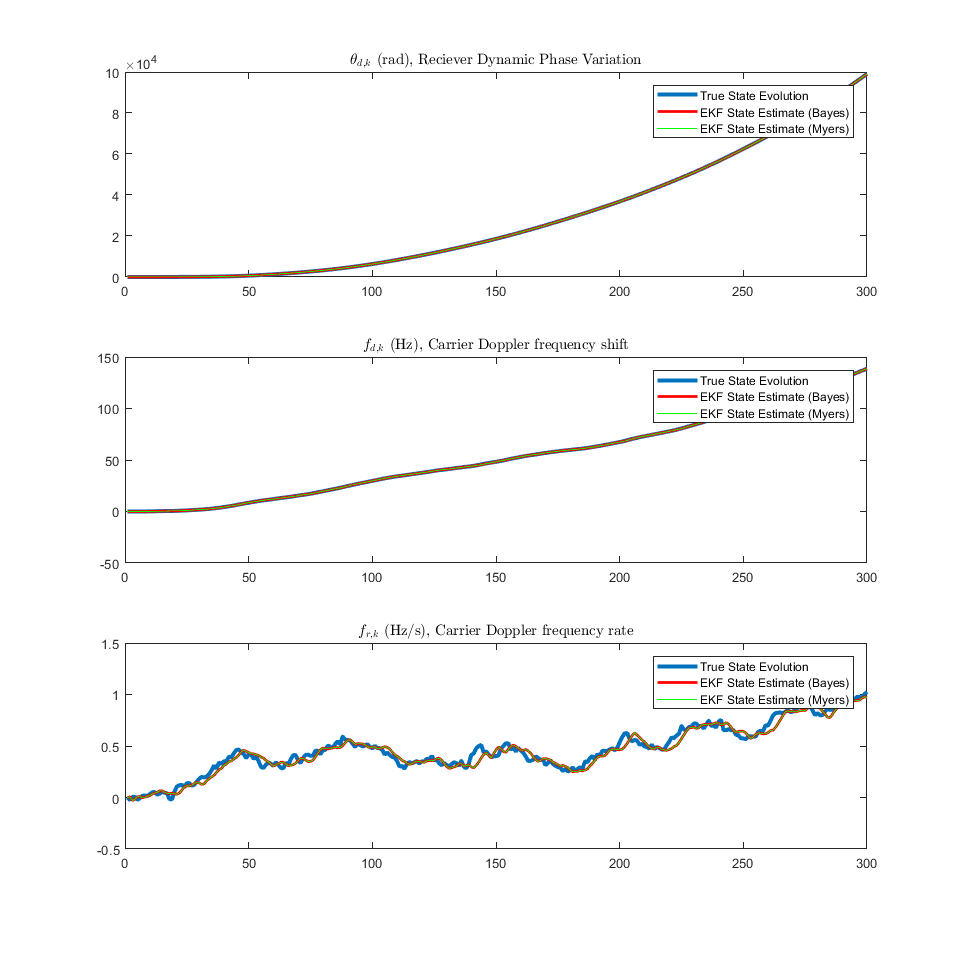
\includegraphics[width=0.8\textwidth]{Final Project/figures/off1.png}
    \caption{True State and Kalman Estimation, Offline Covariance Estimation}
    \label{fig:off1}
\end{figure*}

\begin{figure*}[ht]
    \centering
    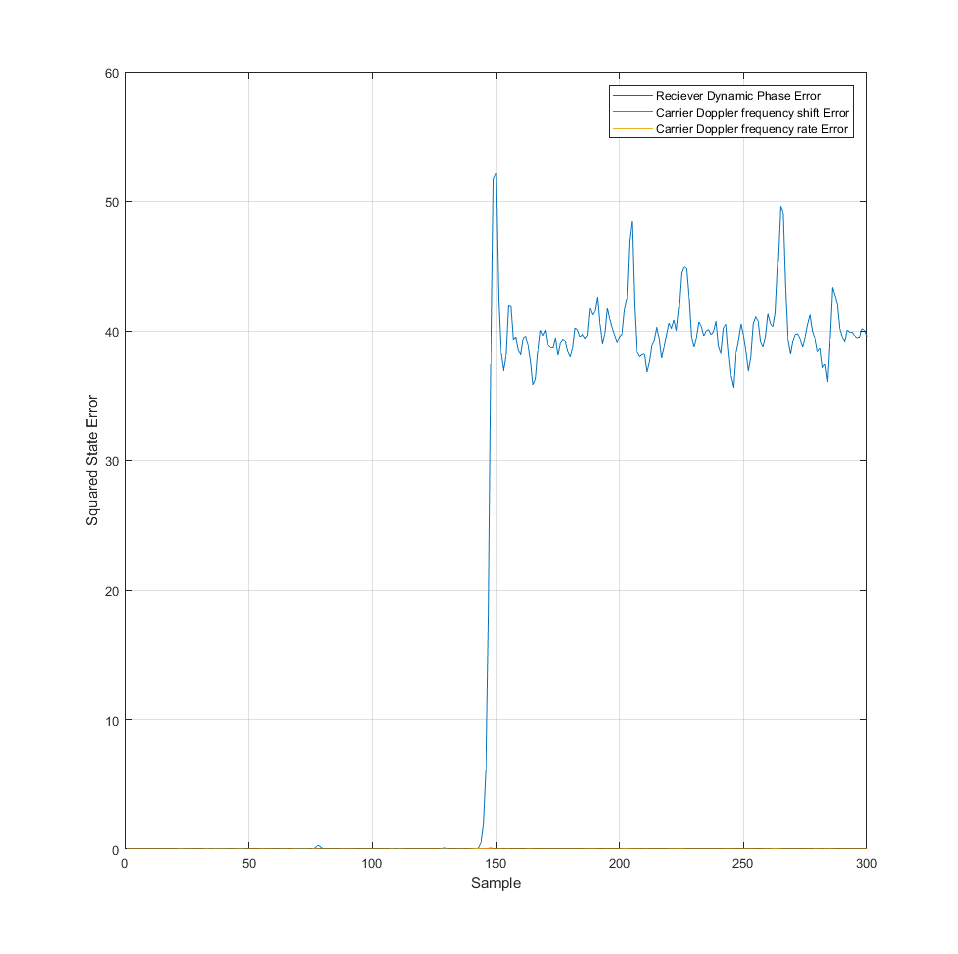
\includegraphics[width=0.8\textwidth]{Final Project/figures/off2.png}
    \caption{True State and Kalman Estimation, Offline Covariance Estimation}
    \label{fig:off2}
\end{figure*}

\begin{figure*}[ht]
    \centering
    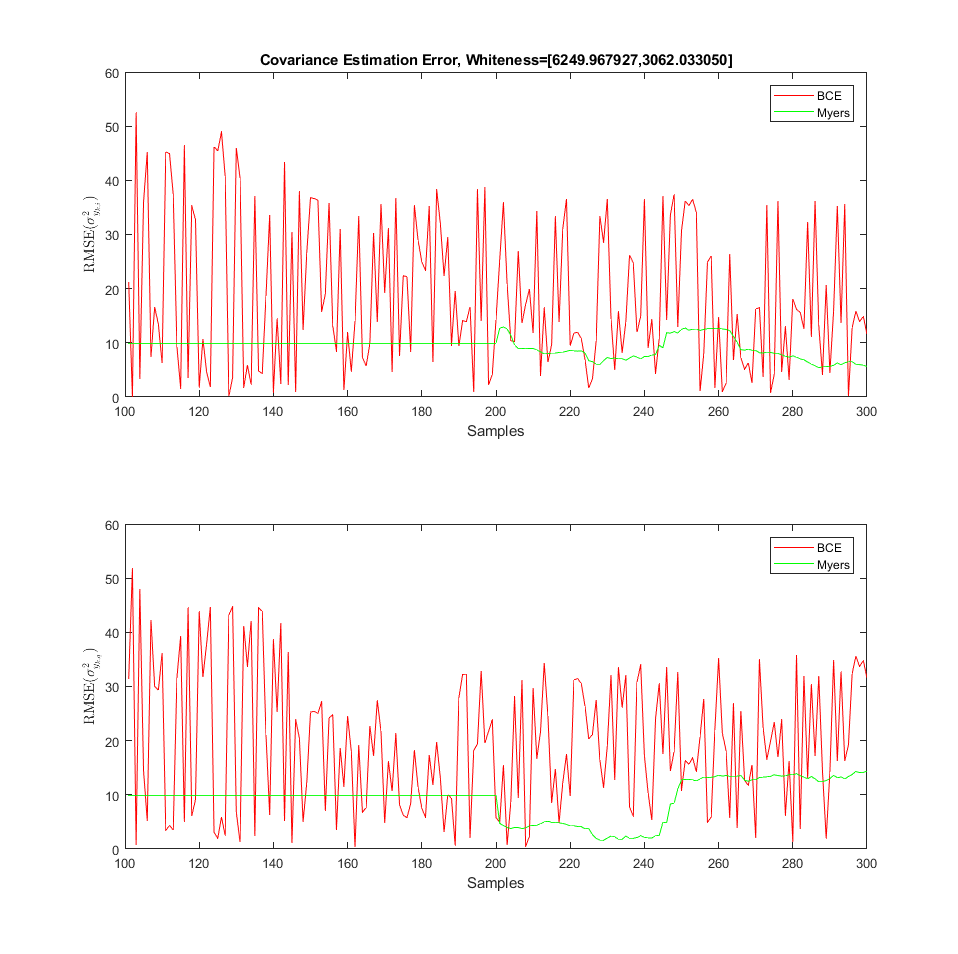
\includegraphics[width=0.8\textwidth]{Final Project/figures/off3.png}
    \caption{True State and Kalman Estimation, Offline Covariance Estimation}
    \label{fig:off3}
\end{figure*}

\begin{figure*}[ht]
    \centering
    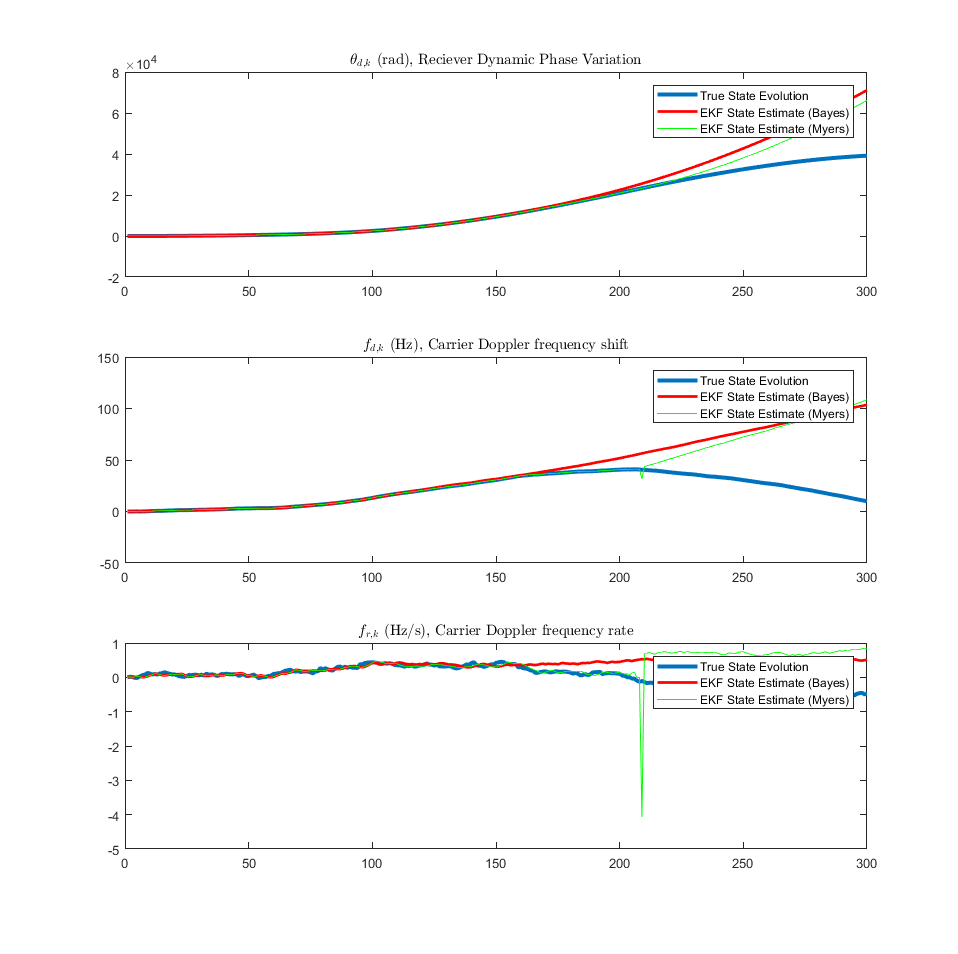
\includegraphics[width=0.8\textwidth]{Final Project/figures/on1.png}
    \caption{True State and Kalman Estimation, Online Covariance Estimation}
    \label{fig:on1}
\end{figure*}

\begin{figure*}[ht]
    \centering
    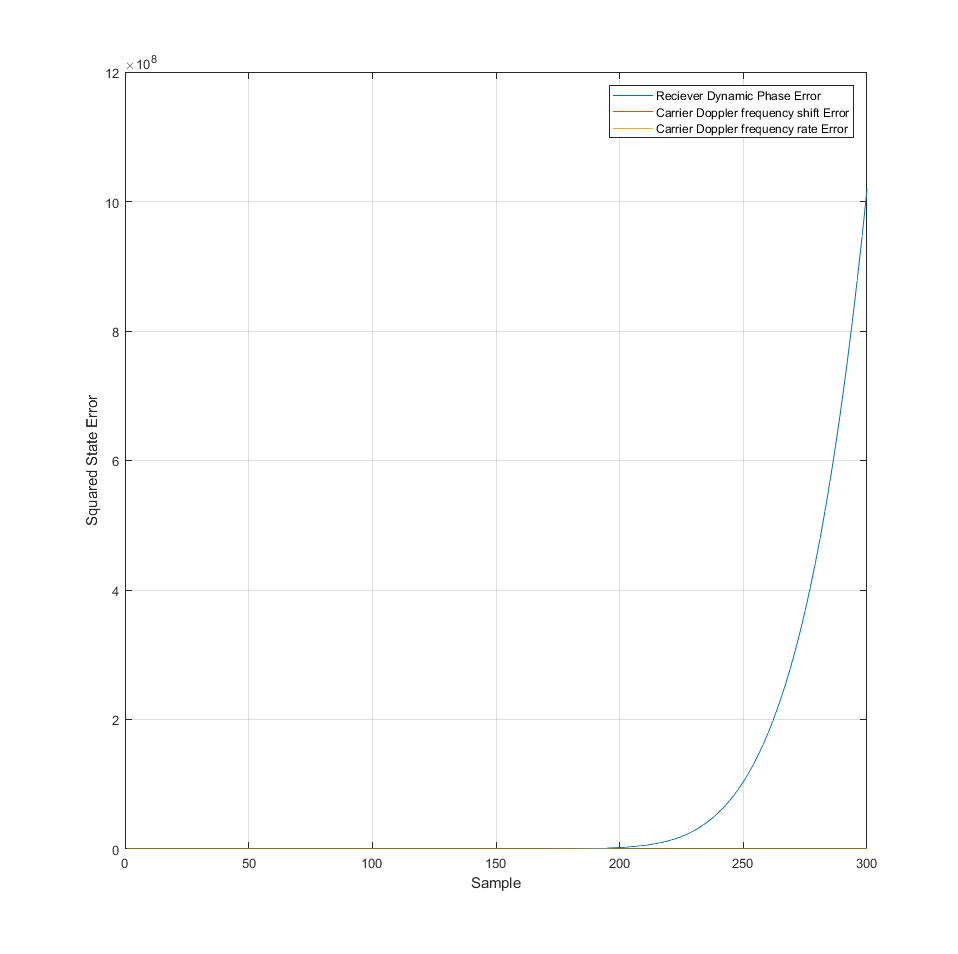
\includegraphics[width=0.8\textwidth]{Final Project/figures/on2.png}
    \caption{True State and Kalman Estimation, Online Covariance Estimation}
    \label{fig:on2}
\end{figure*}

\begin{figure*}[ht]
    \centering
    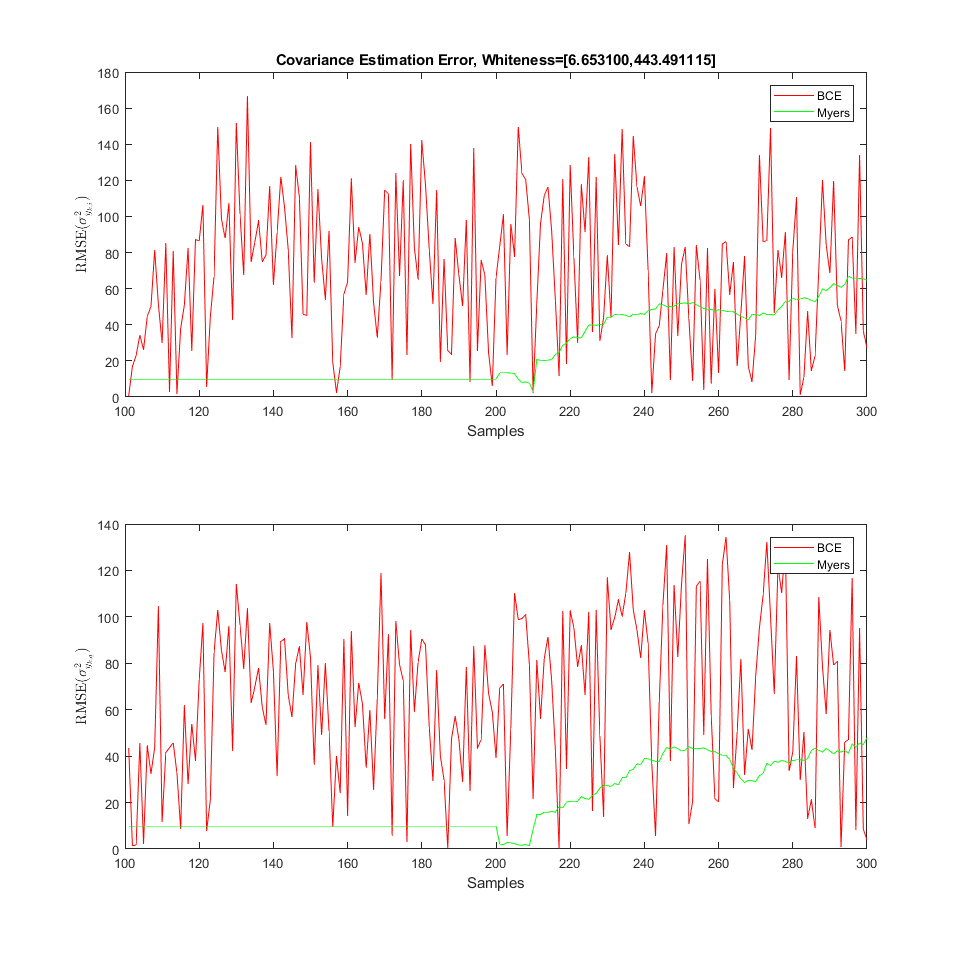
\includegraphics[width=0.8\textwidth]{Final Project/figures/on3.png}
    \caption{True State and Kalman Estimation, Online Covariance Estimation}
    \label{fig:on3}
\end{figure*}

\end{document}